\section{Auswertung}

Die in der Auswertung bestimmten Ausgleichsrechnungen werden mit
dem Python Paket \emph{scipy.optimize}\cite{scipy} durchgeführt.
Desweiten werden die Fehler und insbesondere die Fehlerfortpflanzungen
mit dem Python Paket \emph{uncertainties}\cite{uncertainties} berechnet.

\subsection{Untersuchung der Zerfallskurve von Indium}
Zunächst muss der Nulleffekt der Umgebeung bestimmt werden.
Nach einer Zeit von $\SI{900}{\second}$ wurden

\begin{equation*}
  N\ua{null}=167.
\end{equation*}

Zerfälle gemessen. Umgerechnet auf $1$ und $240$ Sekunden ergibt sich:

\begin{equation}
  \label{eq:nulleffekt_indium}
  N\ua{null,1}=\frac{167}{900} \qquad N\ua{null,240}=\frac{668}{15}.
\end{equation}

Anschließend wird die Aktivität von der Indium-Probe untersucht.
Als Resultat ergeben sich die in \ref{tab: indium_messwerte} aufgelistetetn Messwerte.
In dieser wurde der Nulleffekt berücksichtigt.
\begin{table}
\centering
\caption{Gemessene Anzahl an Zerfällen bei Indium.}
\label{tab: indium_messwerte}
\begin{tabular}{S S S S S }
\toprule
{$t$ in $\si{\second}$} & {Anzahl $N$} & {$\sigma\ua{N}$} & {$\sigma\ua{ln,+}(N)$} & {$\sigma\ua{ln,-}(N)$}  \\
\midrule
 240  & 1914  & 44  & 0.02  & 0.02\\
480  & 1771  & 42  & 0.02  & 0.02\\
720  & 1687  & 41  & 0.02  & 0.02\\
960  & 1665  & 41  & 0.02  & 0.02\\
1200  & 1577  & 40  & 0.02  & 0.03\\
1440  & 1461  & 38  & 0.03  & 0.03\\
1680  & 1491  & 39  & 0.03  & 0.03\\
1920  & 1319  & 36  & 0.03  & 0.03\\
2160  & 1361  & 37  & 0.03  & 0.03\\
2400  & 1233  & 35  & 0.03  & 0.03\\
2640  & 1225  & 35  & 0.03  & 0.03\\
2880  & 1141  & 34  & 0.03  & 0.03\\
3120  & 1062  & 33  & 0.03  & 0.03\\
3360  & 1026  & 32  & 0.03  & 0.03\\
3600  & 948  & 31  & 0.03  & 0.03\\
\bottomrule
\end{tabular}
\end{table}


Die graphische Darstellung ist in Abbildung \ref{fig: plot_indium} zufinden. Bei dieser wurde
die Anzahl $N$ logarithmiert, um einen linearen Zusammenhang aufzuzeigen (vgl. \eqref{eq: zerfallsgesetz}).
\begin{figure}
  \centering
  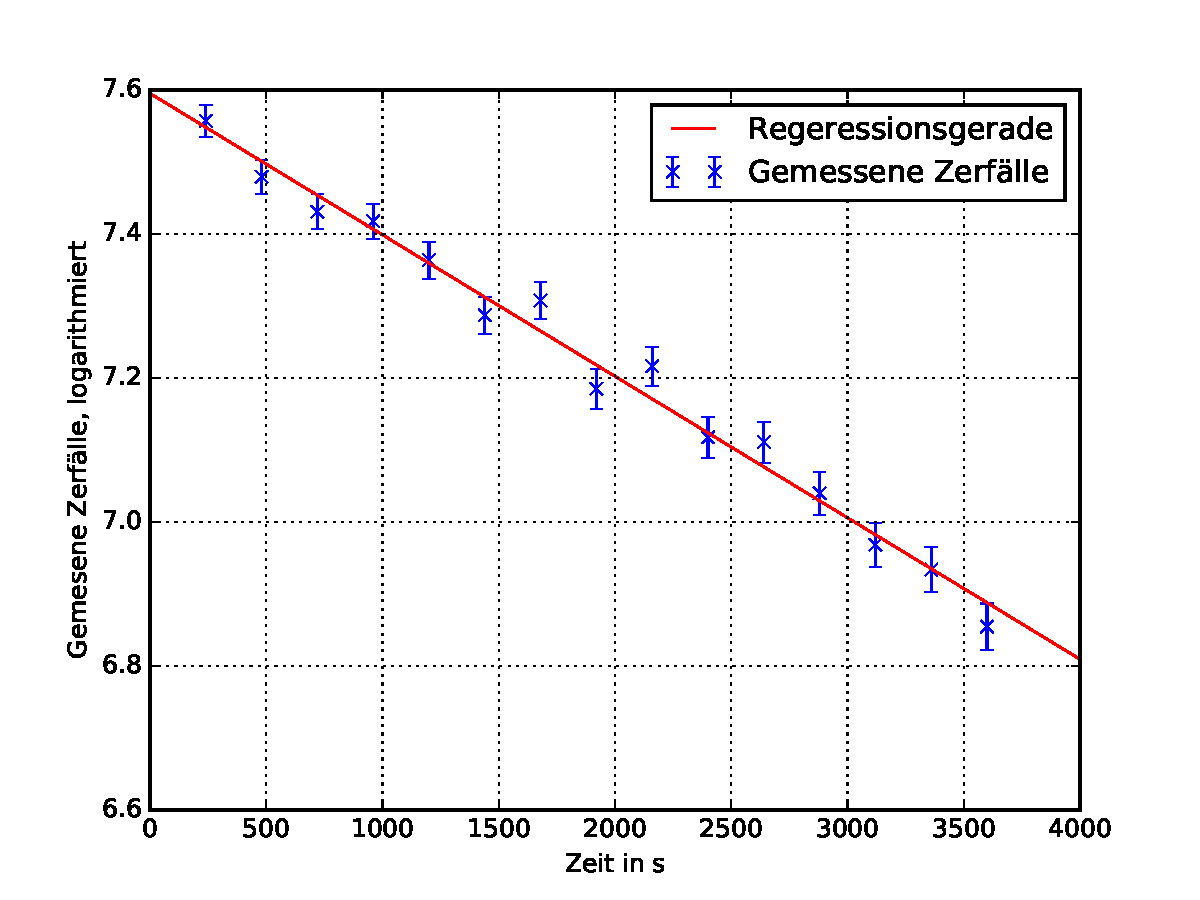
\includegraphics[width=0.8\textwidth]{pics/logarithmiert_indium.pdf}
  \caption{Logarmirierte Darstellung der gemessen Zählraten von Indium und linearer Fit  (unter Berücksichtigung des Nulleffektes).}
  \label{fig: plot_indium}
\end{figure}

Der lineare Zusammenhang kann mit Hilfe von
\begin{equation*}
  g(x)=mx+a
\end{equation*}
notiert werden.
Aus der Regressionrechnung erhält man für die in \ref{fig: plot_indium} zusehende
Ausgleichsgerade die folgenden Parameter:

\begin{align}
  \label{eq:parameter_indium}
  \begin{aligned}
    m\ua{indium}&=\SI{-0.000196\pm0.000007}{\per\second}\\
    a\ua{indium}&=7.595\pm0.015.
  \end{aligned}
\end{align}

Die Parameter aus \eqref{eq:parameter_indium} können in den direkt Zusammenhang mit
\eqref{eq: n_prozeitintervall} gebracht werden. Und zwar gilt:

\begin{align}
  \label{eq:parameter_indium}
  \begin{aligned}
    m\ua{indium}&\Leftrightarrow -\lambda\ua{indium} \quad \Rightarrow \quad \lambda\ua{indium}=\SI{0.000196\pm0.000007}{\per\second}\\
    a\ua{indium}&\Leftrightarrow \ln(b)\ua{indium} \quad \Rightarrow \quad b\ua{indium} =1989\pm 29.
  \end{aligned}
\end{align}

Mit dem Wert für $\lambda\ua{indium}$ und \eqref{eq: halbwertszeit} kann dann die Halbwertszeit von Indium
berechnet weden:

\begin{equation}
  \label{eq:halbwertzeit_indium}
  T\ua{indium}=\SI{3.53\pm0.12 e+3}{\second}
\end{equation}

Im Gegensatz dazu, liegt der Theoriewert für die Halbwertszeit von Indium\cite{indium_halb} bei
\begin{equation}
  \label{eq:halbwertzeit_indium_theo}
  T\ua{indium,theo}=\SI{3.24 e+3}{\second}.
\end{equation}

\subsection{Untersuchung der Zerfallskurve von einem Rhodiumisomer}
